\Chapter{Szürkeárnyalatos képek kiszínezése}

A szürkeárnyalatos kép és a megkapott címke térkép segítségével már az előző fejezetben ki tudtuk színezni a szegmenseket, viszont a kiszínezés az eredeti kép árnyalatait nem vette figyelembe. A fejezet célja hogy a színezést úgy valósítsuk meg, hogy az eredeti kép árnyalatait is megjelenítjük. A minél jobb eredmény elérésének érdekében az RGB és HSV színterekben is megvizsgáltam a problémát, ezeknek a vizsgálatoknak az eredménye a következő alfejezetekben található.

Maguk a színterek a színek matematikai ábrázolásai, lehetővé teszik a színek reprodukálható geometriai ábrázolását a 2D-3D terekben. A színterek a színmodellek és a leképezési függvények kombinációja, és információt tartalmaznak a kép egyes pixeleinek a színéről. A színes képek szegmentálására használt gyakori színterek az RGB, YIQ, HSV, CIE XYZ. \cite{colorspaces}

\Section{RGB}

Az RGB színterű képekben a kép minden egyes pixelét 3 színnel határozzuk meg:
\begin{itemize}
\item vörös (Red)
\item zöld (Green)
\item kék (Blue)
\end{itemize}
A paraméterek a szín intenzitását határozzák meg, az értékük egy 0-255 közötti egész szám. Ha mindegyik paraméterből a maximális, 255 értéket vesszük akkor a fehér színt, ha mindegyikből a minimális, az az a 0 értéket vesszük, akkor pedig a fekete színt kapjuk meg.  Egyszerűsége miatt a színtér széles körben elterjedt. \cite{colorspaces}

Szürkeárnyalatos képek esetén a 3 paraméter értéke megegyezik, így legtöbb esetben csak 1 értékkel szokták a kép pixeleit jelölni, tehát például szürkeárnyalatos képnél egy fekete színű pixel értéke 0. 

Ahhoz, hogy egy szürkeárnyalatos képen színt tudjunk megjeleníteni, először át kell alakítanunk RGB színterűvé. Az átalakítást, hasonlóan az előző fejezetben bemutatott \texttt{color\_image} függvényhez, a \texttt{cv2} csomag \texttt{cvtColor} metódusával fogjuk megtenni.
\begin{python}
colored_image = cv2.cvtColor(resized_image, cv2.COLOR_GRAY2RGB)
\end{python}

Egy adott pixelre a színt a következő képlettel határozom meg:
\begin{align*}
 \text{new\_pixel\_color} & = (R, G, B) \\
 Y & = \text{grayscale\_image}[i][j]\\
 R_{ij} & = Y \cdot R / 255 \\
 G_{ij} & = Y \cdot G / 255 \\
 B_{ij} & = Y \cdot B / 255 \\
 \text{colored\_image}_{ij} & = (R_{ij}, G_{ij}, B_{ij})
\end{align*}
\noindent ahol az $i,j$ a kép adott pixelének az indexe.

A pixeleket a \texttt{numpy} csomag \texttt{multiply} függvényével színezem ki a következő kódrészletben látható módon.

\begin{python}
r, g, b = cv2.split(colored_image)

for i in range(0, k):
    np.multiply(r, colors[i][0]/255, out=r,
                where=label_map==i, casting="unsafe")
    np.multiply(g, colors[i][1]/255, out=g,
                where=label_map==i, casting="unsafe")
    np.multiply(b, colors[i][2]/255, out=b,
                where=label_map==i, casting="unsafe")

colored_image = cv2.merge([r, g, b])
\end{python}

Első lépésként a képet a \texttt{cv2.split} segítségével szétválasztom R, G és B komponensekre. Eredményül 3 tömböt kapok, amik az eredeti pixel adott paraméterét tartalmazzák. Ezeken a tömbökön for ciklus segítségével is végig iterálhatnék, és megadhatnám minden pixelnek az értékét a fentebb említett képlet alapján, viszont a \texttt{numpy} csomag \texttt{multiply} függvénye ezt a szorzást sokkal gyorsabban elvégzi. A klaszterek számán haladok végig, ami tulajdonképpen a címkék értékét jelenti és minden címkére elvégzem a szorzást.

A \texttt{multiply} függvény első 2 paramétereként a szorzás 2 tényezőjét várja. Első elemnek az adott komponens tömböt adom meg, második elemnek pedig a címke által meghatározott szín megfelelő komponensének a 255-el osztott értékét. A \texttt{colors} tömb megegyezik a már korábban bemutatott \texttt{color\_image} függvényben található azonos nevű tömbbel. 

A művelet kimeneti értékének ugyanazt a tömböt adom meg. A szorzásnak megadok egy \texttt{where} feltételt, ahol a címke térkép adott elemét fogja vizsgálni a metódus. Megnézi, hogy az adott címke értéke megegyzik-e az éppen vizsgált címkének az értékével és ha igen, csak akkor végzi el a szorzást, tehát csak akkor színezi ki a pixelt.

Utolsó paraméterként a \texttt{casting} paraméternek unsafe értéket állítok be, ez azt jelenti, hogy a nem egyforma típusú értékek esetén is elvégzi a szorzást a függvény. 

A szorzások után már csak össze kell olvasztanom a 3 különálló tömböt. Ez a \texttt{cv2.merge} függvénnyel egyszerűen megtudom valósítani. A színezésre példa az \ref{fig:colorized_rgb}.ábrán látható. 

\begin{figure}[h]
\centering
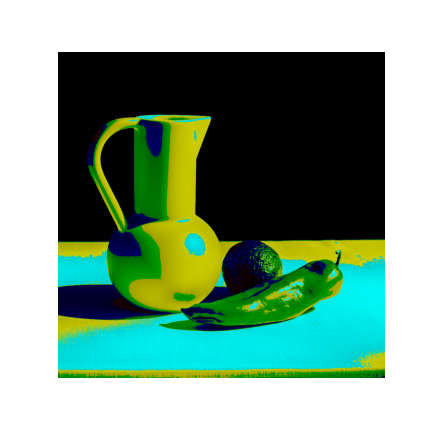
\includegraphics[scale=0.7]{images/colorized_rgb.png}
\caption{Szürkeárnyalatos kép kiszínezése RGB színtérben.}
\label{fig:colorized_rgb}
\end{figure}

Itt már szépen megjelennek az árnyékok, jól kivehetőek a színátmenetek. 

\Section{HSV}